\documentclass[11pt,letterpaper]{article}
\usepackage{xcolor}
\usepackage{textcomp,marvosym}
\usepackage{amsmath,amssymb}
\usepackage[left]{lineno}
\usepackage{changepage}
\usepackage{rotating}
\usepackage{natbib}
\usepackage{setspace}
\usepackage{fancyhdr}
\usepackage{graphicx}
\usepackage{sidecap}
\usepackage{pdfpages}
\usepackage{longtable}

\usepackage[aboveskip=1pt,labelfont=bf,labelsep=period,justification=raggedright,singlelinecheck=off]{caption}
%\doublespacing

\raggedright
\textwidth = 6.5 in
\textheight = 8.5 in
\oddsidemargin = 0.0 in
\evensidemargin = 0.0 in
\topmargin = -0.5 in
\headheight = 0.0 in
\headsep = 0.5 in
\parskip = 0.0 in
\parindent = 0.2 in

%\pagestyle{myheadings}
%\pagestyle{fancy}
%\fancyhf{}
%\lhead{Data Repository (Rapid emplacement of massive Duluth Complex intrusions)}
%\rhead{\thepage}

\begin{document}
\renewcommand{\thefigure}{SI\arabic{figure}}

\subsection*{Supporting Information for ``The paleogeography of Laurentia in its early years: new constraints from the Paleoproterozoic East Central Minnesota batholith''}

\subsubsection*{CA-TIMS U-Pb zircon geochronology methods}

U-Pb dates were obtained by chemical abrasion isotope dilution thermal ionization mass spectrometry (CA-TIMS) in the Boise State University (BSU) Isotope Geology Laboratory (Table DR1; Fig. \ref{fig:zircon_concordia}). Chemical abrasion of single zircon grains was modified after \cite{Mattinson2005a}. Zircons were separated from rocks using standard techniques, annealed in a muffle furnace at 900\textdegree C for 60 hours in quartz crucibles, and imaged by cathodoluminescence in grain mounts (Fig. \ref{fig:zircon_CL}). 

\begin{figure}[!ht]
\noindent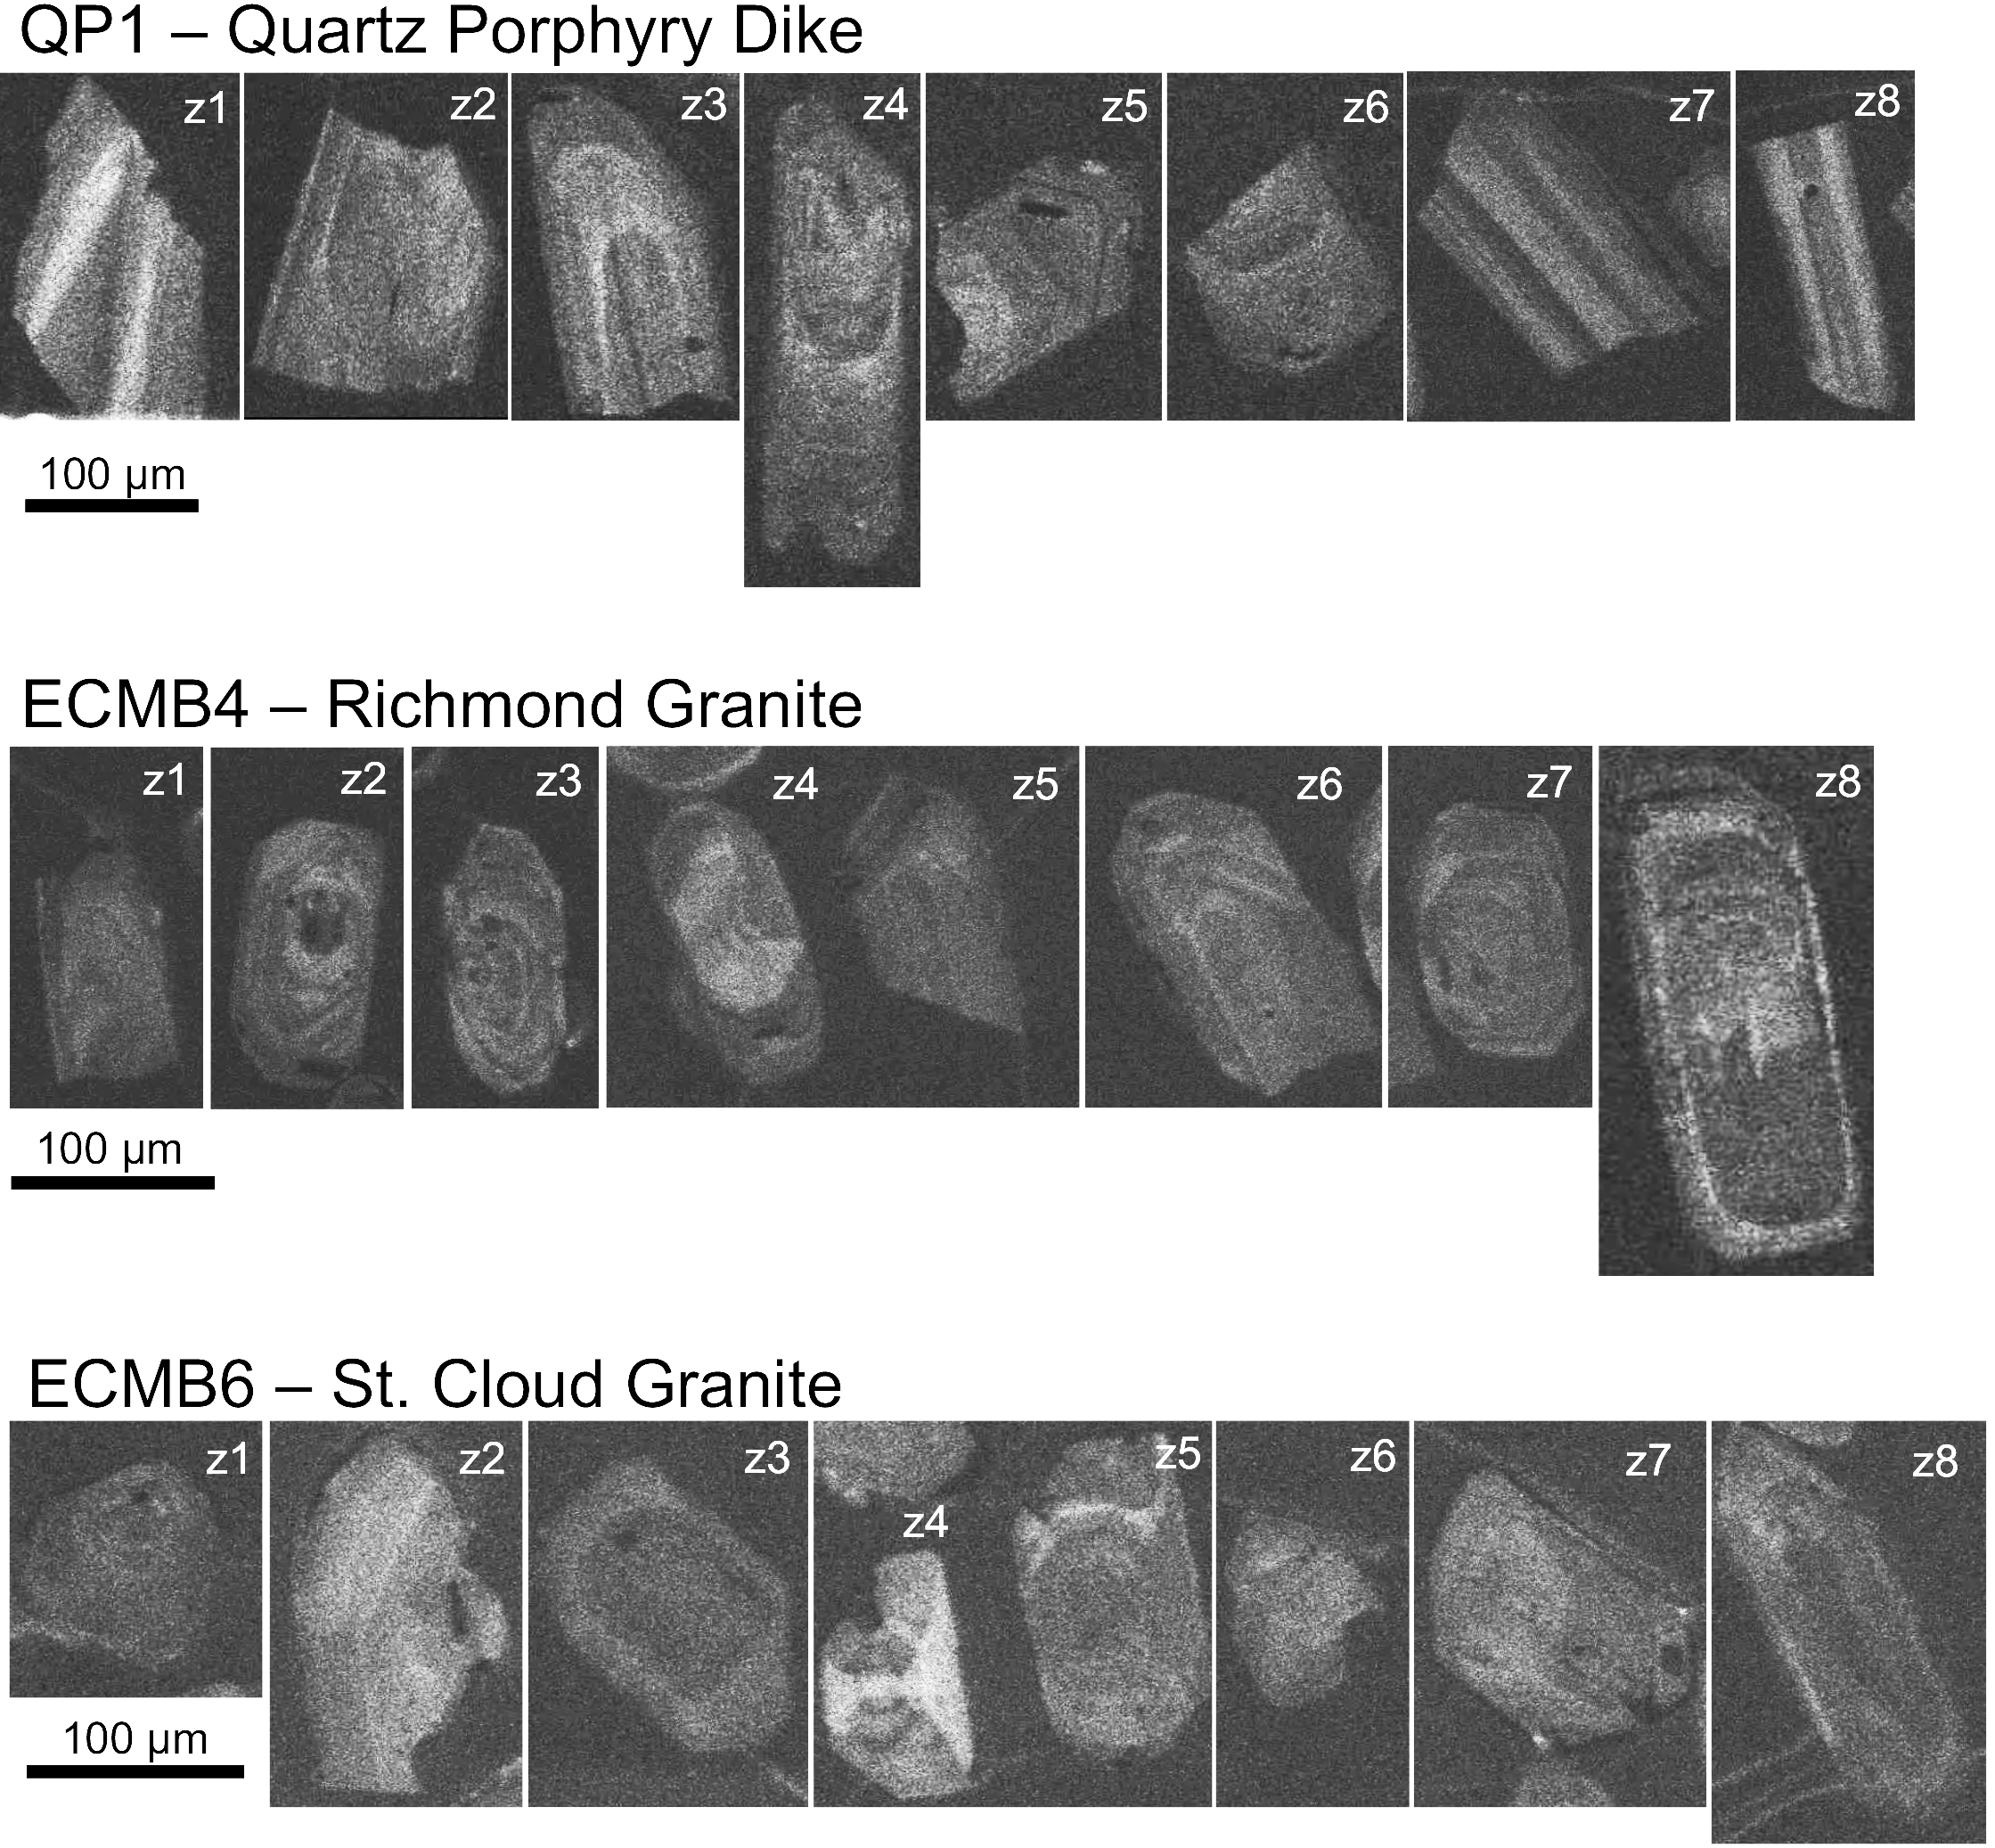
\includegraphics[width=0.8\textwidth]{./figures/SI_zircon_CLimages.png}
\centering
\caption{\small{Cathodoluminescence (CL) images of the zircons dated by ID-TIMS. The 100 $\mu$m scale bars applies for all imaged grains in a given sample.}}
\label{fig:zircon_CL}
\end{figure}

Individual zircons were removed from grain mounts and chemically abraded. Chemical abrasion was carried out by transferring zircons to 3 ml Teflon Perfluoroalkoxy alkane (PFA) beakers in which they were rinsed in 3.5 M HNO$_\mathrm{3}$ and ultrapure H$_\mathrm{2}$O prior to loading into 300 $\mu$l Teflon PFA microcapsules. Fifteen microcapsules were placed in a large-capacity Parr vessel and the zircon partially dissolved in 120 $\mu$l of 29 M HF for 12 hours at 190\textdegree C. Zircons were returned to 3 ml Teflon PFA beakers, HF was removed, and zircons were immersed in 3.5 M HNO$_\mathrm{3}$, ultrasonically cleaned for an hour, and fluxed on a hotplate at 80°C for an hour. The HNO$_\mathrm{3}$ was removed and zircon was rinsed twice in ultrapure H2O before being reloaded into the 300 $\mu$l Teflon PFA microcapsules (rinsed and fluxed in 6 M HCl during sonication and washing of the zircons) and spiked with the $^{233}$U-$^{235}$U-$^{205}$Pb BSU tracer solution (BSU1B). Zircons were dissolved in Parr vessels in 120 $\mu$l of 29 M HF at 220\textdegree C for 48 hours, dried to fluorides, and re-dissolved in 6 M HCl at 180\textdegree C overnight. Pb and U were separated from the zircon matrix using an HCl-based anion-exchange chromatographic procedure \citep{Krogh1973a}, eluted together and dried with 2 $\mu$l of 0.05 N H$_\mathrm{3}$PO$_\mathrm{4}$.

Pb and U were loaded on a single outgassed Re filament in 5 $\mu$l of a silica-gel/phosphoric acid mixture \citep{Gerstenberger1997a}, and Pb and U isotopic measurements made on a GV Isoprobe-T multicollector thermal ionization mass spectrometer equipped with an ion-counting Daly detector. Pb isotopes were measured by peak-jumping all isotopes on the Daly detector for 190 cycles with a mass bias correction of 0.16 $\pm$ 0.03$\%$/a.m.u. (1$\sigma$). Transitory isobaric interferences due to high-molecular weight organics, particularly on $^{204}$Pb and $^{207}$Pb, disappeared within 30-45 cycles, while ionization efficiency averaged 104 cps/pg of each Pb isotope. Linearity (to $\geq$1.4 x 10$^6$ cps) and the associated deadtime correction of the Daly detector were determined by analysis of NBS982. Uranium was analyzed as UO$_2^+$ ions in static Faraday mode on 10$^{12}$ ohm resistors for up to 300 cycles, and corrected for isobaric interference of $^{233}$U$^{18}$O$^{16}$O on $^{235}$U$^{16}$O$^{16}$O with an $^{18}$O/$^{16}$O of 0.00206. Ionization efficiency averaged 20 mV/ng of each U isotope. U mass fractionation was corrected using the $^{233}$U/$^{235}$U ratio of the BSU1B tracer. 

\begin{figure}[!ht]
\noindent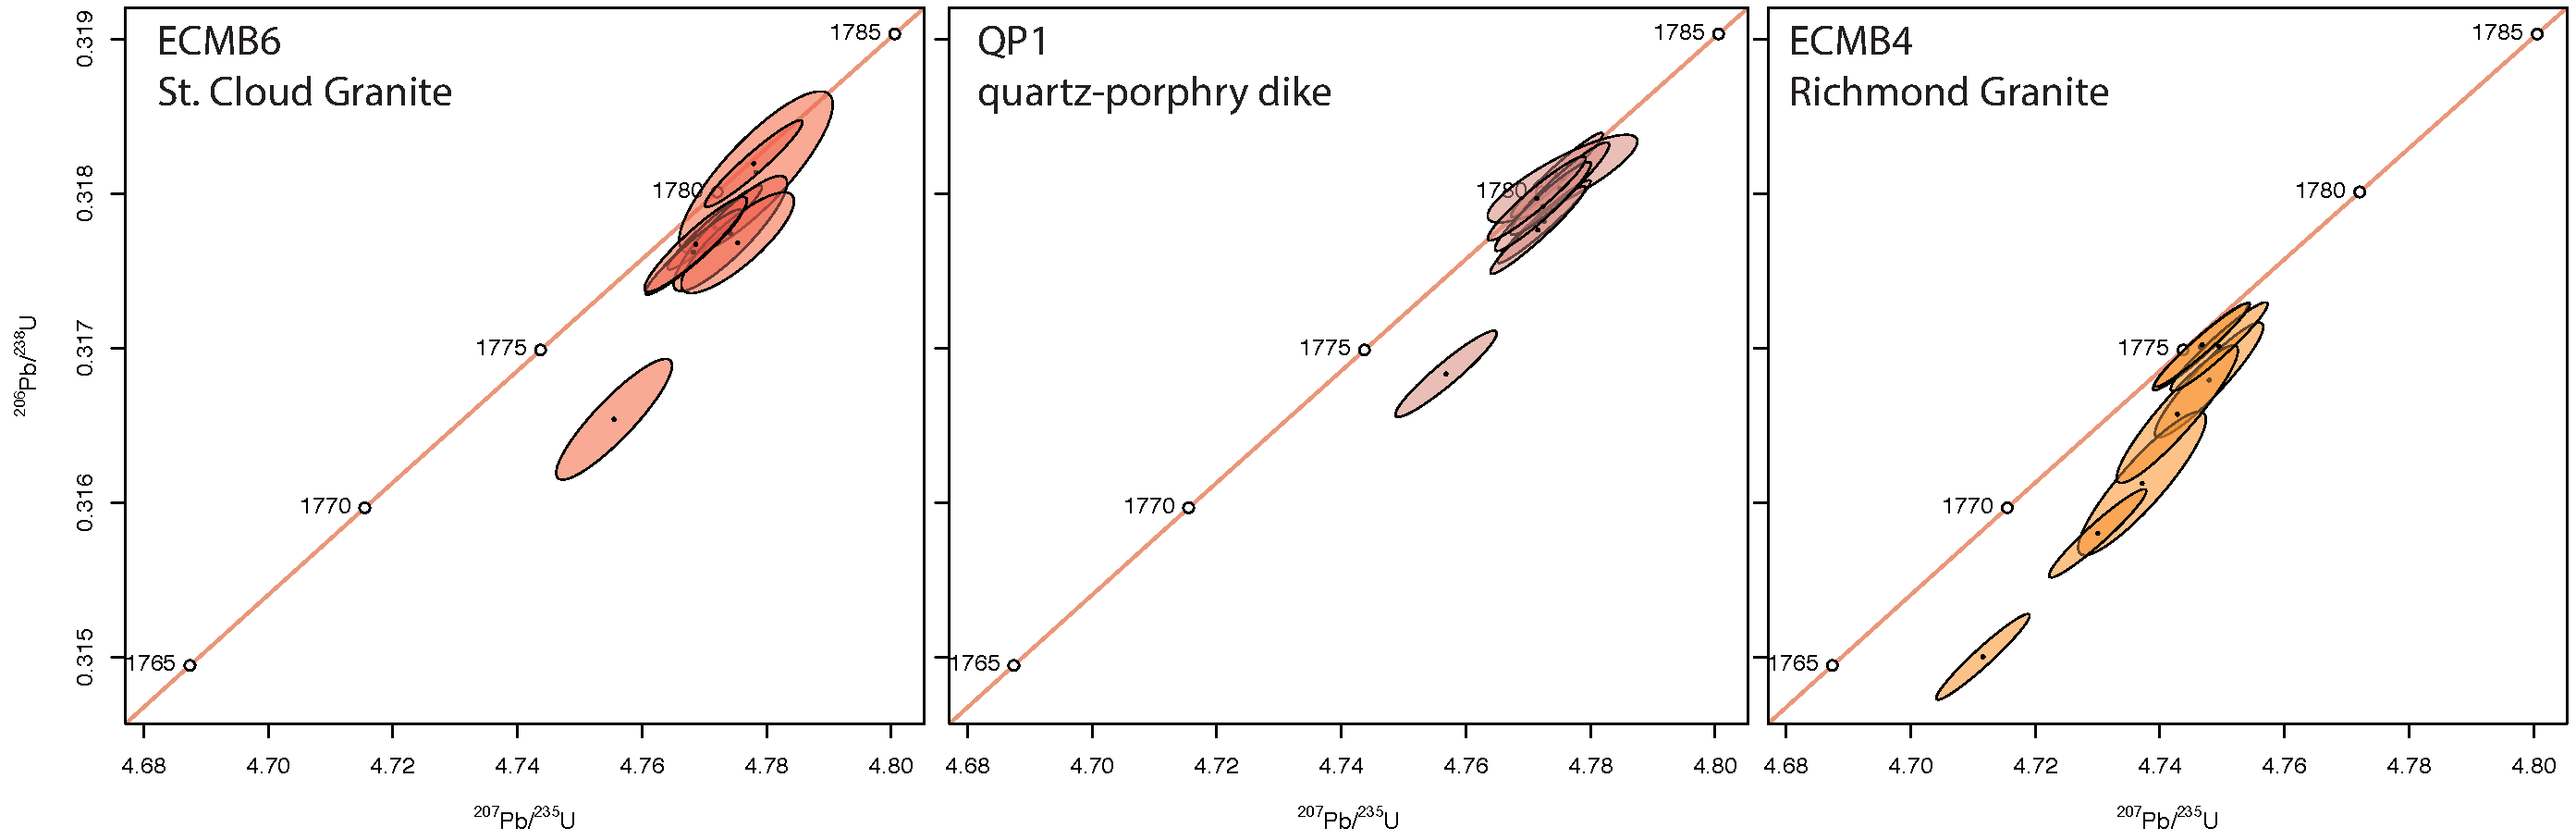
\includegraphics[width=\textwidth]{./figures/SI_zircon_concordia.pdf}
\centering
\caption{\small{U-Pb concordia plots for the new zircon dates. Ellipses represent  2$\sigma$ analytical uncertainty on individual zircon dates.}}
\label{fig:zircon_concordia}
\end{figure}

CA-TIMS U-Pb dates and uncertainties were calculated using the algorithms of \cite{Schmitz2007b}, BSU1B tracer solution with calibration of $^{235}$U/$^{205}$Pb = 77.93 and $^{233}$U/$^{235}$ = 1.007066, and U decay constants recommended by \cite{Hiess2012a}, including $^{238U}$/$^{235}$U of 137.818. $^{206}$Pb/$^{238}$U ratios and dates were corrected for initial $^{230}$Th disequilibrium using DTh/U = 0.20 $\pm$ 0.05 (1$\sigma$). All common Pb in analyses was attributed to laboratory blank and subtracted based on the measured laboratory Pb isotopic composition and associated uncertainty. U blanks are estimated at 0.013 pg. CA-TIMS weighted mean $^{207}$Pb/$^{206}$Pb dates were calculated from equivalent dates (pof $>$0.05) using Isoplot 3.0 \citep{Ludwig2003a}. Errors on the weighted mean dates are given as $\pm$ x / z, where x is the internal error based on analytical uncertainties including counting statistics, subtraction of tracer solution, and blank and initial common Pb subtraction; z also includes the U decay constant uncertainties propagated in quadrature. Dates from individual zircon fractions and weighted mean dates are reported at 2$\sigma$.

\subsubsection*{LA-ICP-MS U-Pb apatite geochronology methods}

Apatite U-Pb geochronology data were developed via laser ablation inductively coupled mass spectrometry (LA-ICP-MS) at UC Santa Barbara. U-Pb isotopes were analyzed with a Cetac Teledyne 193 nm excimer Analyte laser with a HelEx ablation cell coupled to a Nu Instruments Plasma 3D multi-collector (MC) ICP-MS. On the Plasma 3D, $^{204}$(Pb+Hg), $^{206}$Pb, $^{207}$Pb, and $^{208}$Pb were measured on Daly detectors and $^{238}$U and $^{232}$Th were measured on Faraday collectors. Apatite was ablated with a 40 $\mu$m diameter laser spot for 60 pulses fired at a 4 Hz repetition rate and 50$\%$ of 5 mJ laser power. Each ablation sequence consisted of 2 cleaning shots, followed by 25 secs of monitored washout and 15 secs of ablation. The Iolite v. 2.5 program \citep{Paton2011a} in the Igor Pro software environment was used to correct the raw U-Pb ratios for baselines, laser- and plasma-induced element fractionation, and instrument drift.

Multiple apatite reference materials (RMs) were analyzed throughout the analytical session to monitor data quality. Apatite RM Madagascar (478.4 $\pm$ 6.1 Ma, ID-TIMS age; \citealp{Thomson2012a}) served as the primary bracketing standard with RMs McClure (523.5 $\pm$ 1.5 Ma, ID-TIMS age; \citealp{Schoene2006a}), 401 (530.3 $\pm$ 1.5 Ma, ID-ICP-MS age; \citealp{Thompson2016a}) and OD306 (1596.7 $\pm$ 7.1 Ma, ID-ICP-MS age; \citealp{Thompson2016a}) analyzed as secondary standards to assess precision and accuracy. All of the secondary standards form mixing arrays between common-Pb and an age intercept. The excess variances of $^{206}$Pb/$^{238}$U and $^{207}$Pb/$^{206}$Pb required for secondary standards to conform to a statistically single mixing line are 2.1$\%$ and 2.0$\%$ (2$\sigma$), respectively; these values were added in quadrature to the internal uncertainties of each U-Pb datum \citep{Horstwood2016a}. The ages of the secondary standards with these designated uncertainties are 547.4 ± 30.4/35.9 Ma (McClure), 512.8 $\pm$ 9.8/10.5 Ma (401), 1586.5 $\pm$ 14.9/15.7 Ma (OD306) (uncertainties following the same format used in main text), within uncertainty of their published ages. Although mass-204 was measured on the MC-ICP-MS, isobaric interferences with $^{204}$Hg in the He carrier gas preclude the use of the $^{204}$Pb method for common-Pb corrections.

\textit{Common-Pb corrections were done using the $^{207}$Pb method (e.g., Ludwig, 2008) and implemented an initial $^{207}$Pb/206Pb ratio derived from regressions through data with enough spread along a mixing line in Concordia space or from a Stacey and Kramers (1975) model at appropriate reference ages. NEED TO REVISIT THIS TEXT}  The U-Pb apatite data are reported in Table S2.


\begin{figure}[!ht]
\noindent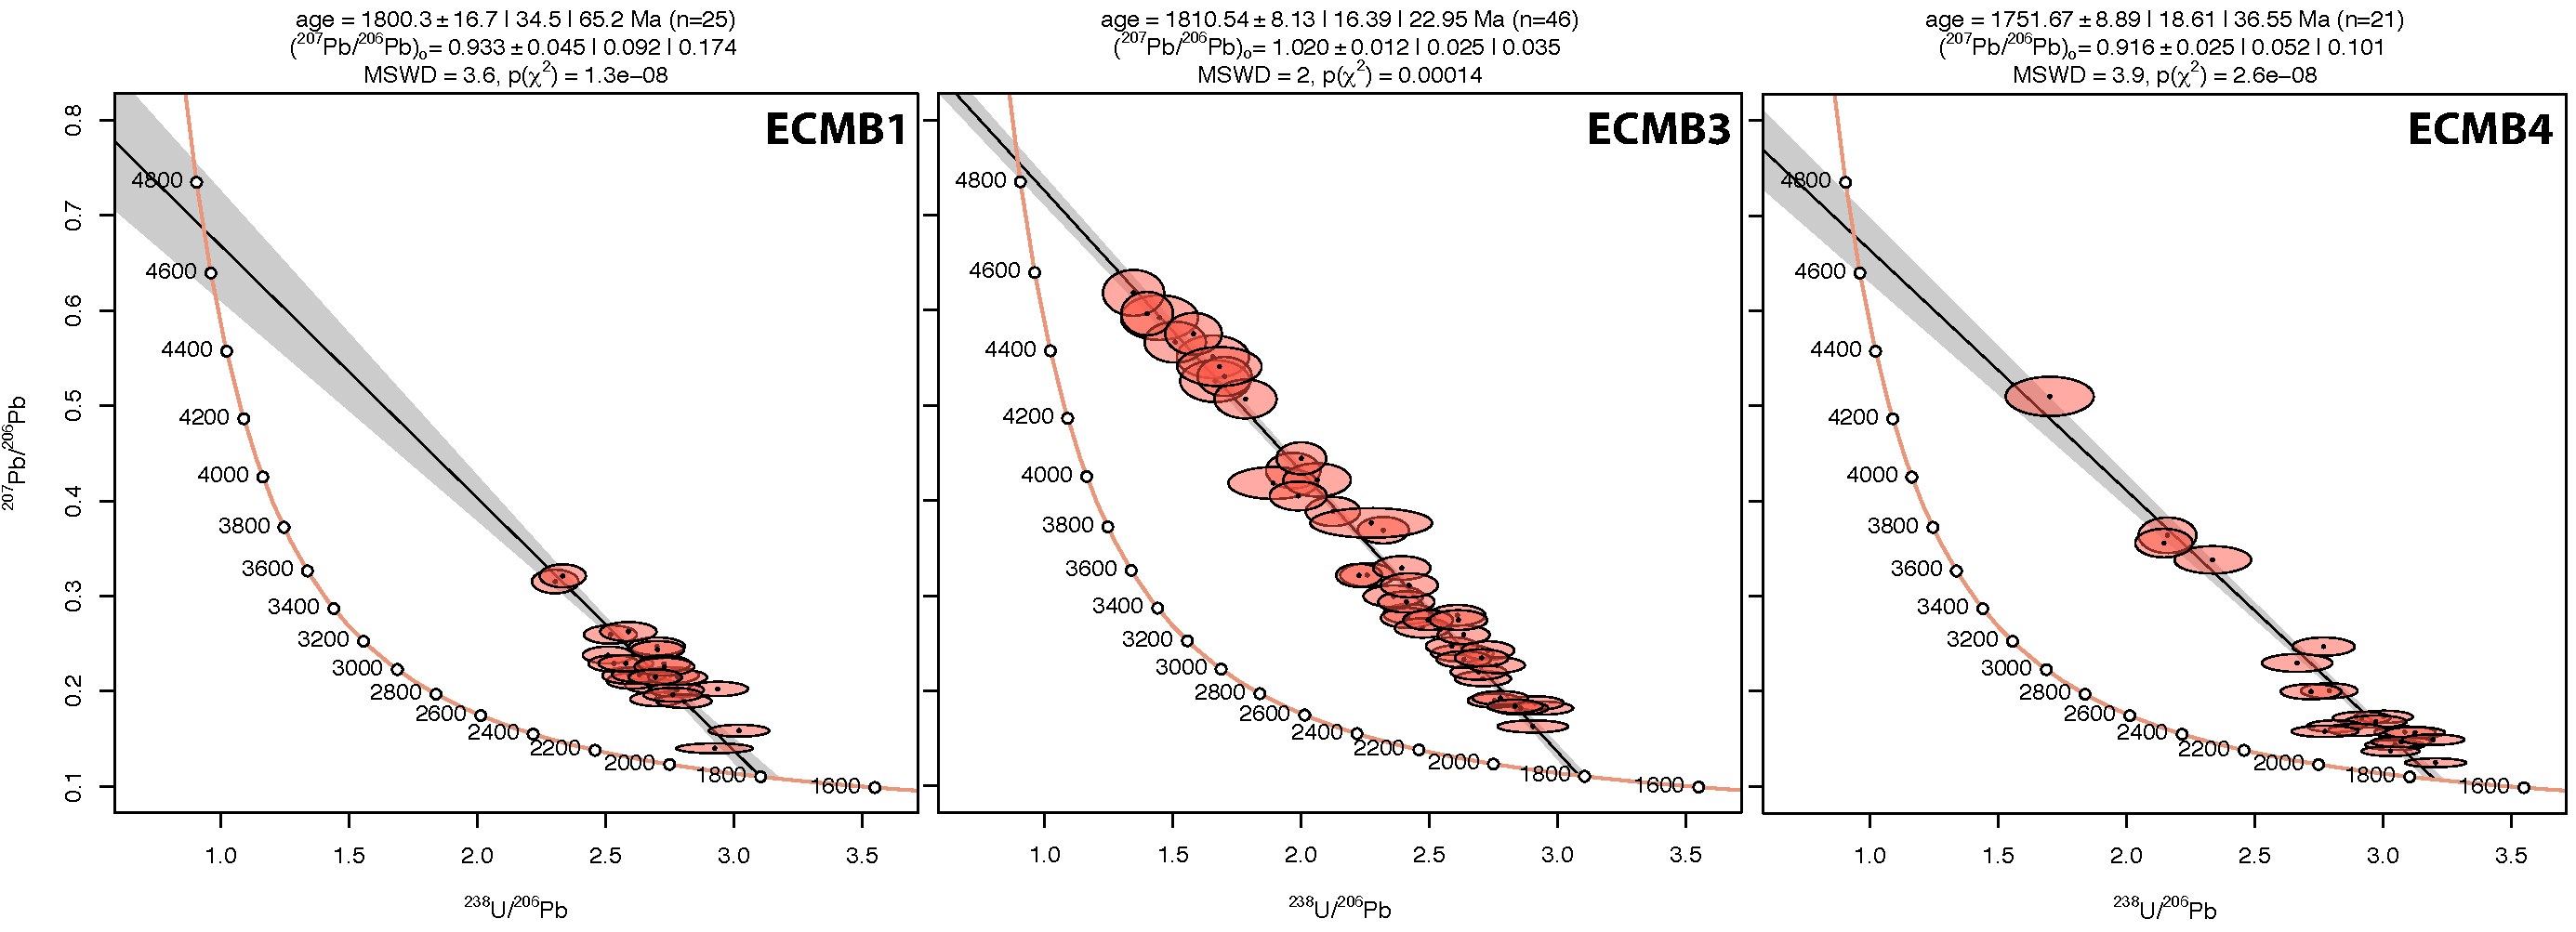
\includegraphics[width=\textwidth]{./figures/SI_apatite_TW.pdf}
\centering
\caption{\small{U-Pb Tera-Wasserburg plots for the new apatite dates. Ellipses represent 2$\sigma$ analytical uncertainty on individual apatite dates. The }}
\label{fig:apatite_TW}
\end{figure}

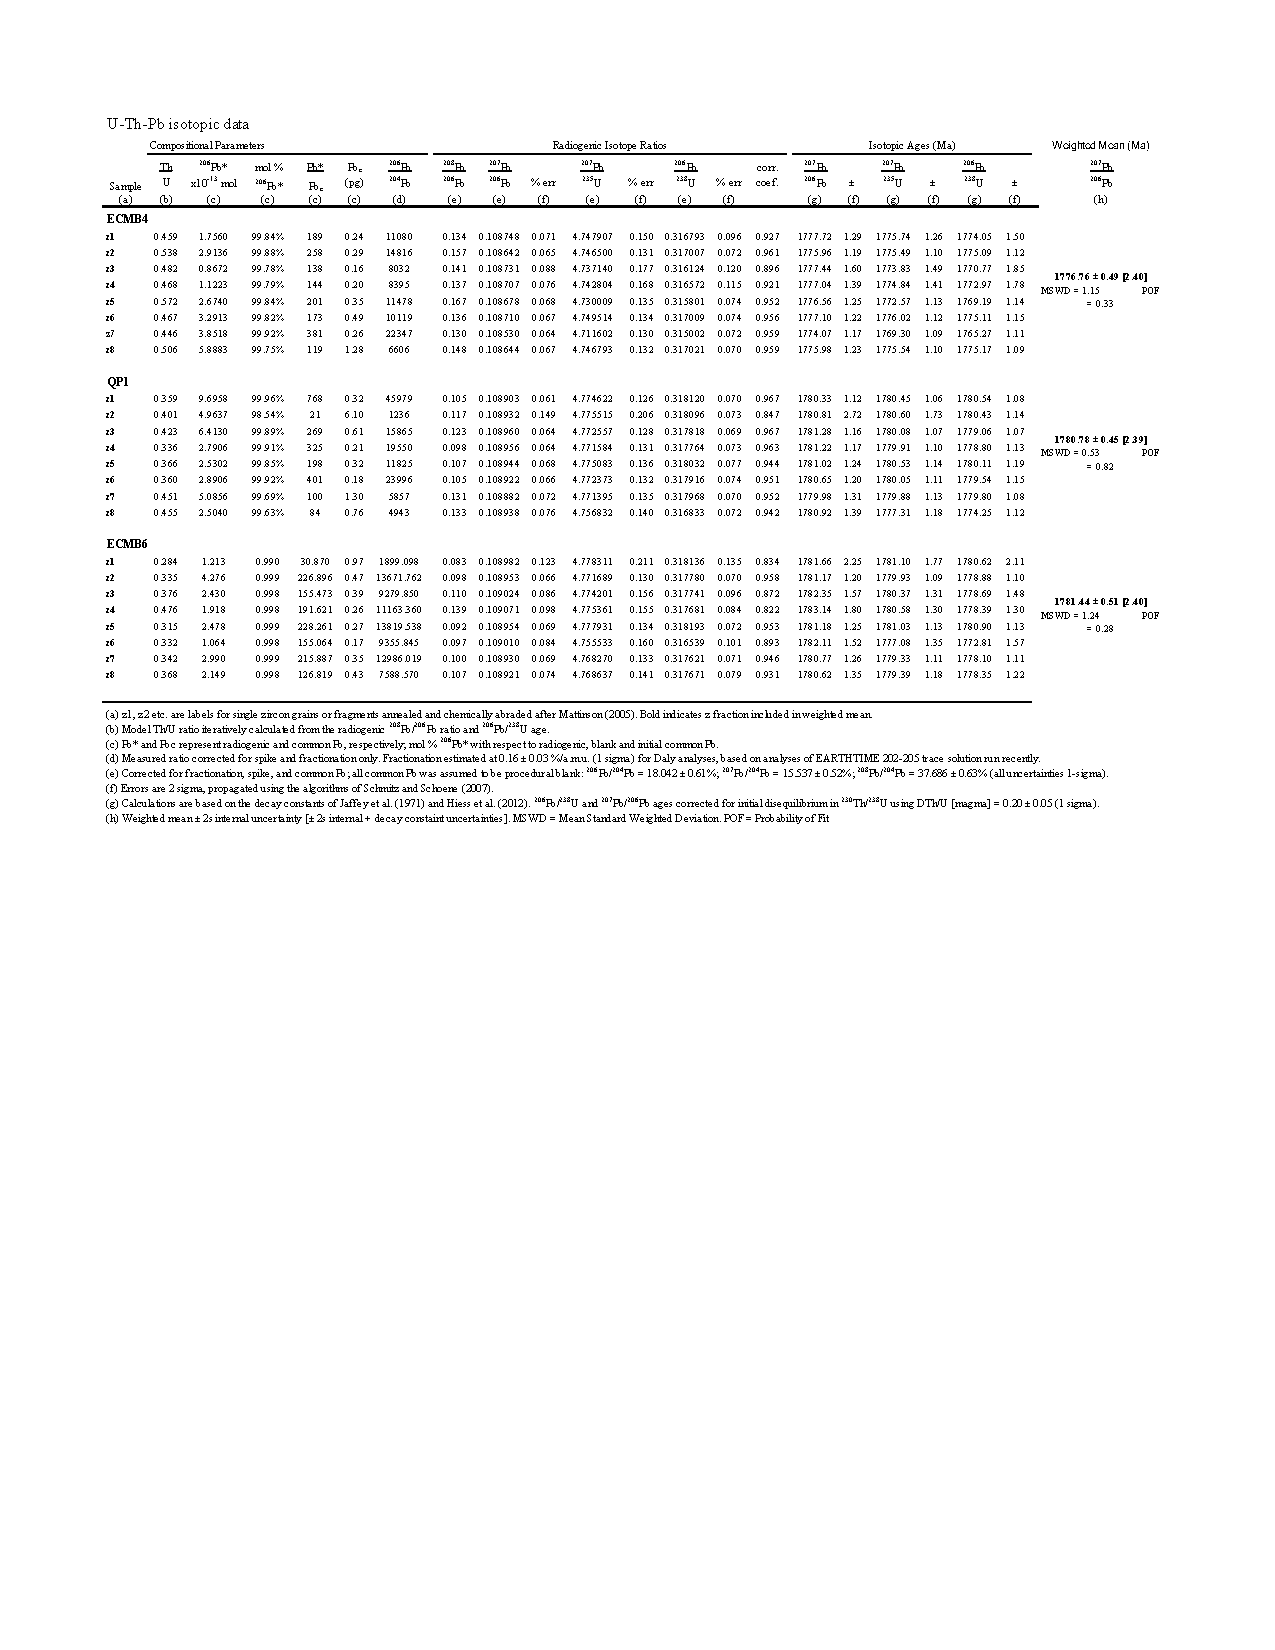
\includepdf[pages=-,pagecommand={},width=7.65 in]{tables/zircon_U_Pb_data_table.pdf}

\begin{table}[h!]
\tiny
\caption{Site level paleomagnetic data}
\begin{tabular}{|l|r|r|r|r|r|r|r|r|r|r|r|}
\hline
site & site lat & site lon & n & dec$_{is}$ & inc$_{is}$ & dec$_{tc}$ & inc$_{tc}$ & k & $\alpha_{95}$ & VGP lat & VGP lon \\
\hline
	FC1 (AF)		&	47.7826	&	-91.3265	&	9	&	301.6	&	40.5	&	297.1	&	52.4	&	32	&	9.3	&	41.3	&	185.0	\\
\textbf{FC1 (thermal)	}	&	47.7826	&	-91.3265	&	9	&	289.7	&	34.4	&	284.1	&	45.1	&	64	&	6.5	&	28.6	&	187.8	\\
\textbf{FC4 (AF)	}	&	47.7625	&	-91.3827	&	7	&	296.0	&	26.8	&	292.6	&	38.3	&	59	&	7.9	&	30.8	&	177.4	\\
	HCT1 (AF)		&	47.6008	&	-91.1495	&	7	&	287.2	&	35.6	&	281.0	&	46.0	&	54	&	8.3	&	26.9	&	190.8	\\
\textbf{HCT1 (thermal)	}	&	47.6008	&	-91.1495	&	6	&	285.7	&	45.3	&	276.3	&	55.3	&	144	&	5.6	&	29.5	&	201.0	\\
\textbf{1 (Beck layered)	}	&	46.68	&	-92.24	&	4	&	279.5	&	47.5	&	287.7	&	64.4	&	51	&	9.8	&	42.0	&	205.2	\\
	3 (Beck layered)		&	46.68	&	-92.24	&	4	&	292.0	&	26.5	&	298.0	&	41.9	&	17	&	17.2	&	36.3	&	175.6	\\
	4 (Beck layered)		&	46.68	&	-92.24	&	3	&	279.5	&	36.0	&	284.5	&	53.0	&	20	&	18.0	&	33.0	&	193.5	\\
	5 (Beck layered)		&	46.68	&	-92.24	&	3	&	279.5	&	55.0	&	291.8	&	71.7	&	14	&	22.0	&	48.4	&	217.4	\\
	6 (Beck layered)		&	46.68	&	-92.24	&	1	&	280.5	&	32.0	&	285.0	&	48.9	&		&		&	31.1	&	189.7	\\
\textbf{7 (Beck layered)	}	&	46.68	&	-92.24	&	5	&	278.0	&	33.0	&	282.0	&	50.1	&	85	&	6.8	&	29.7	&	192.7	\\
\textbf{8 (Beck layered)	}	&	46.68	&	-92.24	&	7	&	290.5	&	43.0	&	301.6	&	58.3	&	345	&	2.8	&	47.5	&	189.4	\\
\textbf{9 (Beck layered)	}	&	46.68	&	-92.23	&	3	&	281.5	&	42.0	&	288.7	&	58.7	&	35	&	13.6	&	39.2	&	197.0	\\
	10 (Beck layered)		&	46.70	&	-92.23	&	3	&	297.5	&	30.5	&	305.6	&	44.9	&	15	&	21.2	&	43.0	&	172.0	\\
	11 (Beck layered)		&	46.70	&	-92.22	&	1	&	284.0	&	30.5	&	289.2	&	47.0	&		&		&	32.9	&	185.6	\\
\textbf{12 (Beck layered)	}	&	46.72	&	-92.21	&	5	&	284.5	&	36.0	&	291.1	&	52.4	&	43	&	9.6	&	37.1	&	188.9	\\
\textbf{13 (Beck layered)	}	&	46.69	&	-92.24	&	6	&	281.5	&	28.0	&	285.6	&	44.8	&	437	&	2.7	&	29.3	&	186.4	\\
\textbf{14 (Beck layered)	}	&	46.72	&	-92.20	&	7	&	287.0	&	35.0	&	294.1	&	51.1	&	334	&	2.9	&	38.4	&	185.8	\\
	15 (Beck layered)		&	46.73	&	-92.21	&	2	&	290.0	&	31.5	&	296.9	&	47.2	&		&		&	38.2	&	180.4	\\
\textbf{17 (Beck layered)	}	&	46.74	&	-92.19	&	3	&	279.5	&	37.0	&	284.7	&	54.0	&	80	&	9.1	&	33.8	&	194.3	\\
\textbf{19 (Beck layered)	}	&	46.75	&	-92.19	&	4	&	288.0	&	35.0	&	295.3	&	50.9	&	51	&	9.8	&	39.2	&	184.8	\\
\textbf{20 (Beck layered)	}	&	46.77	&	-92.15	&	3	&	282.0	&	33.0	&	287.1	&	49.7	&	444	&	3.8	&	33.0	&	189.1	\\
	25 (Beck layered)		&	46.78	&	-92.12	&	1	&	273.5	&	18.5	&	274.9	&	36.0	&		&		&	17.7	&	188.5	\\
	27 (Beck layered)		&	46.77	&	-92.15	&	1	&	310.0	&	40.5	&	324.6	&	51.6	&		&		&	59.4	&	162.2	\\
	30 (Beck layered)		&	46.77	&	-92.14	&	1	&	284.0	&	36.5	&	290.6	&	53.0	&		&		&	37.1	&	189.8	\\
	32 (Beck layered)		&	46.77	&	-92.14	&	1	&	290.0	&	36.0	&	298.2	&	51.6	&		&		&	41.5	&	183.5	\\
	33 (Beck layered)		&	46.77	&	-92.15	&	2	&	288.0	&	32.0	&	294.5	&	48.0	&		&		&	37.0	&	182.7	\\
\textbf{35 (Beck layered)	}	&	46.79	&	-92.23	&	8	&	290.0	&	23.5	&	294.9	&	39.3	&	194	&	3.6	&	32.9	&	176.1	\\
	36 (Beck layered)		&	46.78	&	-92.21	&	2	&	276.0	&	27.0	&	278.6	&	44.3	&		&		&	24.3	&	190.6	\\
	37 (Beck layered)		&	46.79	&	-92.25	&	2	&	273.0	&	29.0	&	275.0	&	46.5	&		&		&	23.1	&	194.3	\\
	92 (Beck layered)		&	46.81	&	-92.10	&	3	&	290.0	&	41.5	&	300.2	&	57.0	&	16	&	20.1	&	45.9	&	188.3	\\
\textbf{93 (Beck layered)	}	&	46.83	&	-92.18	&	5	&	284.5	&	24.5	&	288.6	&	41.0	&	151	&	5.1	&	29.4	&	181.7	\\
\textbf{94 (Beck layered)	}	&	46.85	&	-92.04	&	4	&	291.0	&	36.5	&	299.6	&	51.9	&	107	&	6.8	&	42.7	&	182.9	\\
	97 (Beck layered)		&	46.78	&	-92.12	&	2	&	281.0	&	28.5	&	285.0	&	45.4	&		&		&	29.2	&	187.2	\\
\textbf{98 (Beck layered)	}	&	46.77	&	-92.13	&	6	&	288.5	&	34.0	&	295.7	&	49.9	&	115	&	5.3	&	38.8	&	183.6	\\
\textbf{99 (Beck layered)	}	&	46.77	&	-92.12	&	3	&	287.0	&	35.0	&	294.1	&	51.1	&	39	&	13.0	&	38.4	&	185.8	\\
	103 (Beck layered)		&	46.75	&	-92.18	&	2	&	276.0	&	29.0	&	278.8	&	46.3	&		&		&	25.5	&	191.8	\\
	215 (Beck layered)		&	48.08	&	-90.77	&	2	&	281.0	&	48.0	&	290.2	&	64.7	&		&		&	44.4	&	204.8	\\
\textbf{217 (Beck layered)	}	&	46.79	&	-92.20	&	5	&	287.0	&	41.0	&	296.0	&	57.0	&	53	&	8.6	&	43.0	&	190.8	\\
\textbf{218 (Beck layered)	}	&	46.79	&	-92.18	&	6	&	284.5	&	27.5	&	289.2	&	44.0	&	62	&	7.3	&	31.3	&	183.3	\\
	219 (Beck layered)		&	46.79	&	-92.17	&	5	&	284.5	&	33.5	&	290.5	&	49.9	&	10	&	19.7	&	35.3	&	187.1	\\
\textbf{220 (Beck layered)	}	&	46.80	&	-92.15	&	5	&	284.0	&	30.5	&	289.2	&	47.0	&	291	&	3.7	&	32.9	&	185.6	\\
\textbf{221 (Beck layered)	}	&	46.79	&	-92.14	&	5	&	290.5	&	27.5	&	296.4	&	43.2	&	1433	&	1.7	&	35.8	&	177.6	\\
\textbf{18 (Beck anorthosite)	}	&	46.75	&	-92.17	&	7	&	279.0	&	37.5	&	284.1	&	54.5	&	91	&	5.5	&	33.7	&	195.2	\\
	21 (Beck anorthosite)		&	46.77	&	-92.15	&	2	&	290.0	&	42.0	&	300.5	&	57.5	&		&		&	46.3	&	188.8	\\
	22 (Beck anorthosite)		&	46.78	&	-92.12	&	6	&	275.0	&	40.5	&	279.1	&	57.8	&	10	&	17.8	&	32.6	&	201.4	\\
	23 (Beck anorthosite)		&	46.78	&	-92.12	&	2	&	295.5	&	39.5	&	306.5	&	54.0	&		&		&	48.5	&	180.6	\\
	26 (Beck anorthosite)		&	46.77	&	-92.15	&	2	&	309.5	&	43.5	&	325.8	&	54.5	&		&		&	61.9	&	165.6	\\
	31 (Beck anorthosite)		&	46.77	&	-92.14	&	1	&	278.0	&	33.0	&	282.0	&	50.1	&		&		&	29.7	&	192.7	\\
	38 (Beck anorthosite)		&	46.83	&	-92.11	&	2	&	262.0	&	33.0	&	260.9	&	50.6	&		&		&	16.7	&	206.2	\\
	40 (Beck anorthosite)		&	46.83	&	-92.09	&	2	&	309.0	&	35.0	&	320.7	&	46.6	&		&		&	54.0	&	160.2	\\
	101 (Beck anorthosite)		&	46.76	&	-92.16	&	2	&	296.5	&	37.5	&	306.9	&	51.9	&		&		&	47.6	&	177.7	\\
	102 (Beck anorthosite)		&	46.75	&	-92.18	&	1	&	275.0	&	29.0	&	277.6	&	46.4	&		&		&	24.7	&	192.7	\\
\textbf{222 (Beck anorthosite)	}	&	46.76	&	-92.15	&	5	&	270.5	&	43.0	&	273.0	&	60.6	&	75	&	7.3	&	30.7	&	207.6	\\
\hline
\end{tabular}
%\begin{tablenotes}[para,flushleft]

Notes: n--number of samples analyzed and included in the site mean; dec-- mean declination for the site (is = insitu; tc = tilt-corrected); inc--mean inclination for the site; k--Fisher precision parameter; $\alpha_{95}$--95$\%$ confidence limit in degrees; VGP lat--latitude of the virtual geomagnetic pole for the site; VGP lon--longitude of the virtual geomagnetic pole for the site. Sites in \textbf{bold} were included in the calculation of the mean pole (filtered for $\alpha_{95}<15^{\circ}$ and so that only one site for FC1 and HCT). The resulting mean pole is: 188.7\textdegree E, 35.6\textdegree N, N=24, A$_{95}$=3.1, k=92.
%\end{tablenotes}
\end{table}

\clearpage
\pagebreak
\singlespacing

\small
\begin{thebibliography}{6}
\providecommand{\natexlab}[1]{#1}
\providecommand{\url}[1]{\texttt{#1}}
\providecommand{\urlprefix}{URL }
\expandafter\ifx\csname urlstyle\endcsname\relax
  \providecommand{\doi}[1]{doi:\discretionary{}{}{}#1}\else
  \providecommand{\doi}{doi:\discretionary{}{}{}\begingroup
  \urlstyle{rm}\Url}\fi

\bibitem[{Gerstenberger and Haase(1997)}]{Gerstenberger1997a}
Gerstenberger, H. and Haase, G., 1997, A highly effective emitter substance for
  mass spectrometric {P}b isotope ratio determinations: Chemical Geology, vol.
  136, pp. 309--312.

\bibitem[{Hiess et~al.(2012)Hiess, Condon, McLean, and Noble}]{Hiess2012a}
Hiess, J., Condon, D.~J., McLean, N., and Noble, S.~R., 2012,
  $^{238}${U}/$^{235}${U} systematics in terrestrial uranium-bearing minerals:
  Science, vol. 335, pp. 1610--1614, \doi{10.1126/science.1215507}.

\bibitem[{Krogh(1973)}]{Krogh1973a}
Krogh, T., 1973, A low contamination method for the hydrothermal decomposition
  of zircon and extraction of {U} and {P}b for isotopic age determinations:
  Geochimica Cosmochimicha Acta, vol.~37, pp. 485--494,
  \doi{10.1016/0016-7037(73)90213-5}.

\bibitem[{Ludwig(2003)}]{Ludwig2003a}
Ludwig, K.~R., 2003, Isoplot 3.0. a geochronological toolkit for {M}icrosoft
  {E}xcel: Tech. rep., Berkeley Geochronology Center.

\bibitem[{Mattinson(2005)}]{Mattinson2005a}
Mattinson, J.~M., 2005, {Zircon U/Pb chemical abrasion (CA-TIMS) method:
  Combined annealing and multi-step partial dissolution analysis for improved
  precision and accuracy of zircon ages}: Chemical Geology, vol. 220, pp.
  47--66, \doi{10.1016/j.chemgeo.2005.03.011}.

\bibitem[{Schmitz and Schoene(2007)}]{Schmitz2007b}
Schmitz, M.~D. and Schoene, B., 2007, {Derivation of isotope ratios, errors,
  and error correlations for U-Pb geochronology using
  $^{205}$Pb-$^{235}$U-($^{233}$U)-spiked isotope dilution thermal ionization
  mass spectrometric data}: Geochem. Geophys. Geosyst., vol.~8, p. Q08,006,
  \doi{10.1029/2006GC001492}.

\end{thebibliography}

%\small
%\nocite{Schmitz2007b}
%\bibliographystyle{gsabull}
%\bibliography{../../../0000_Github/references/allrefs}

\end{document}
